\chapter{Evaluation}
\label{c:eval}

This chapter discuss the n-to-n evaluation of our system.

\section{Evaluation dataset}
\label{s:eval}
For collecting the ground truth data we walked along the path of 300 feet at an urban street to record the video with samrtphone.
We record data at different time of the day and at different light condition.
\ref{f:dataset} shows the scene variation of recored video.
The right one is cloudy and the left one is sunny.

\begin{figure}[!ht]
\centering
\subfloat[Sunny] {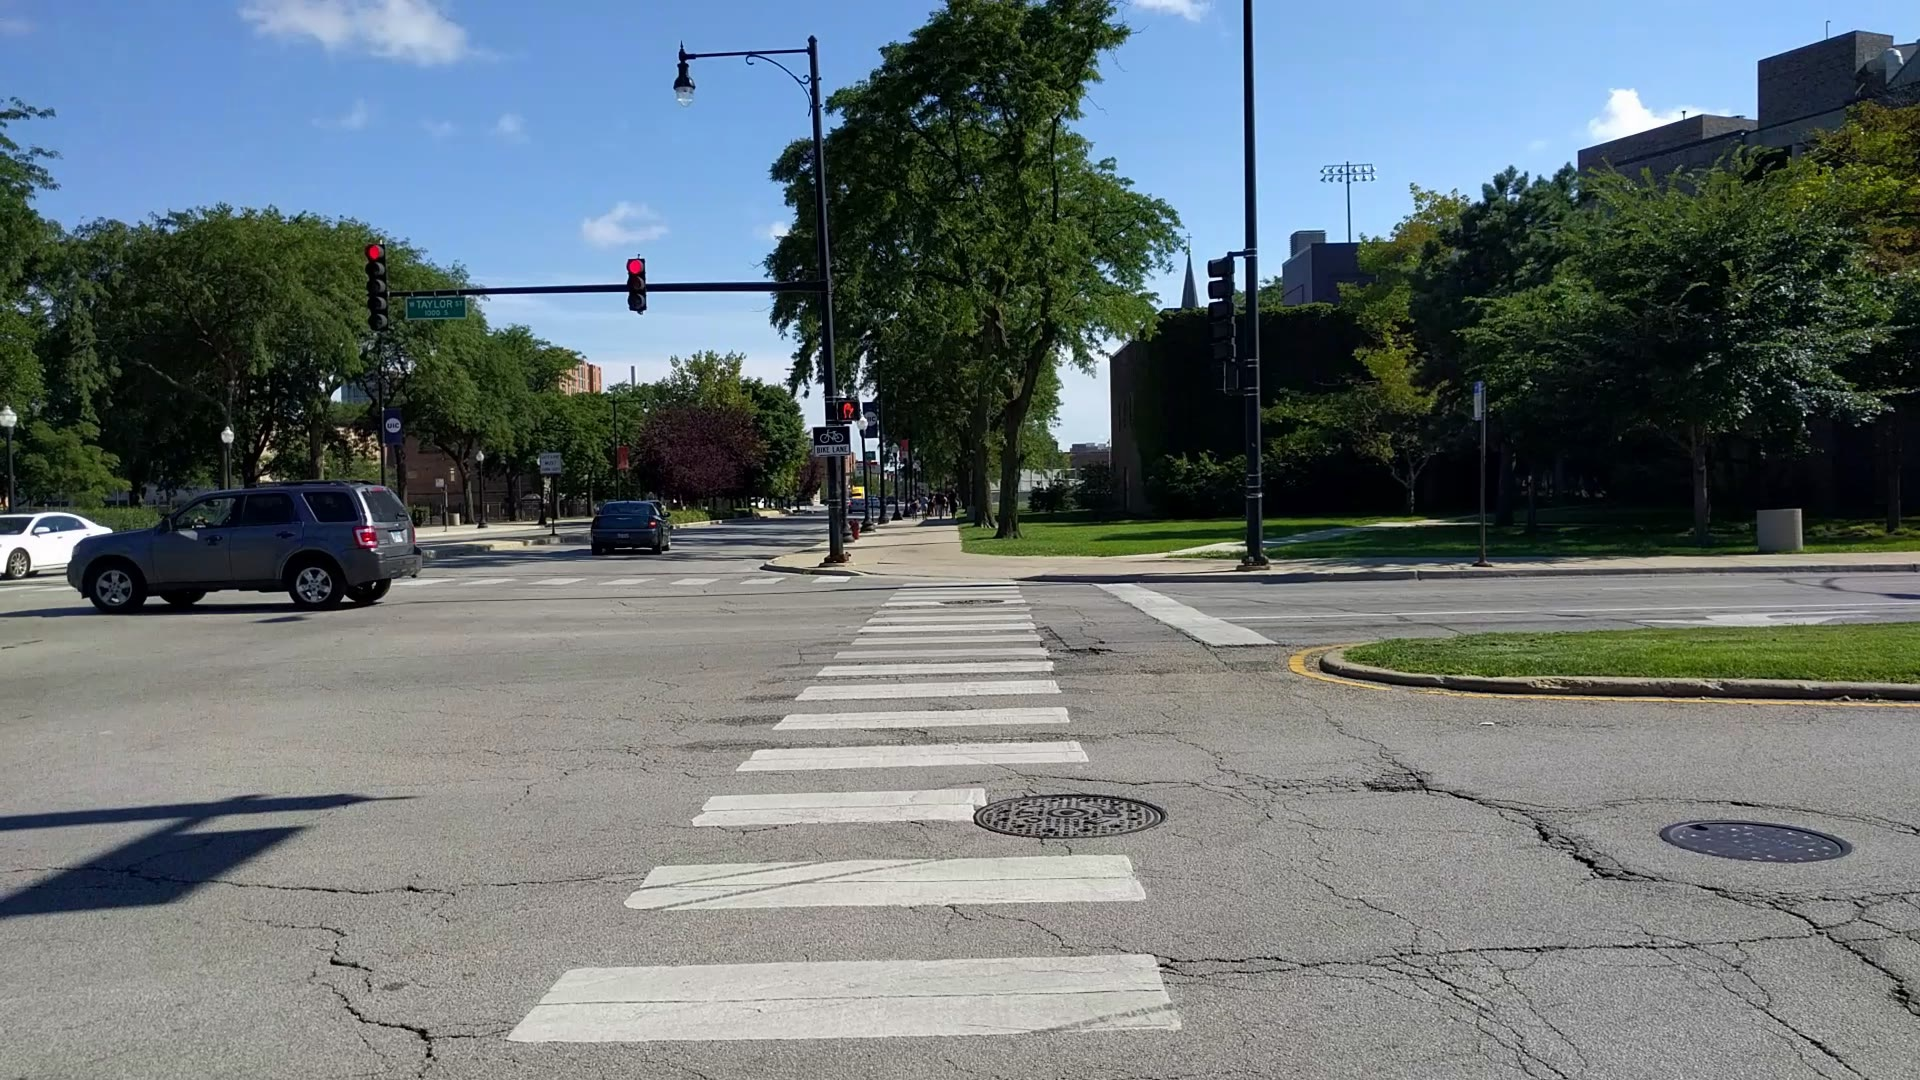
\includegraphics[width=3in]{images/sunny.jpg}}
\hfill
\subfloat[Cloudy] {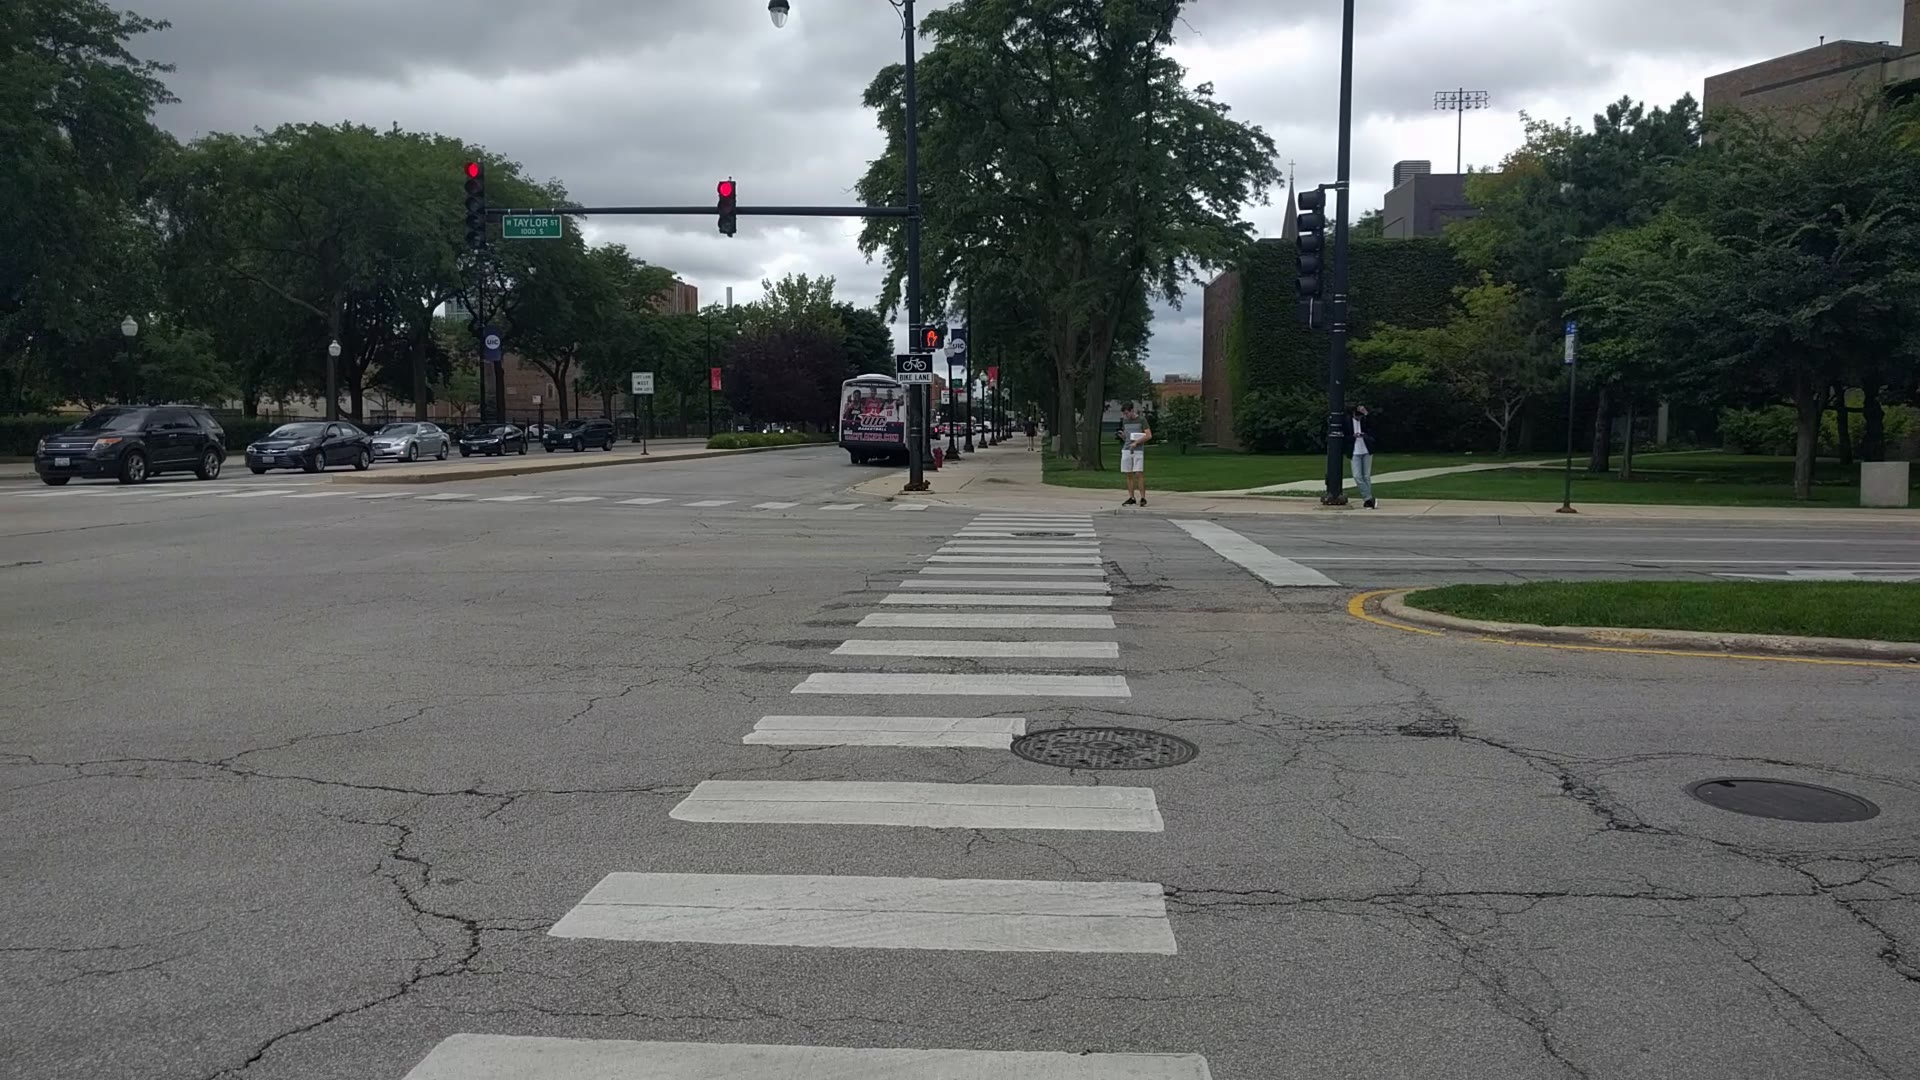
\includegraphics[width=3in]{images/cloudy.jpg}}

\caption{Scene variation of recorded video.}
\label{f:dataset}
\end{figure}

\ref{t:dataset} shows the total no of frames, and time duration of our dataset.

\begin{table}[h!]
  \centering
  \caption{Description of the dataset.}
  \label{t:dataset}
  \begin{tabular}{  l  c  r  }
   
    Name & Frame Count & Time Duration \\
    \hline
    Walk with sensor movement-Sunny day & 5905 & 3 mins 16 secs  \\
    Walk with sensor movement-Cloudy day & 6205 & 3 mins 26 secs \\
    Walk regular movement & 6022 & 3 mins 20 secs \\
    Static with sensor movement & 1810 & 1 min 
    \hline
  \end{tabular}
\end{table}

\section{Computation time}
We collected data at different time of the day as we discussed in \ref{s:eval}.
In this section we discuss the processing time of these dataset with the sensor hint and without it.

\begin{figure}[h!]
\centering
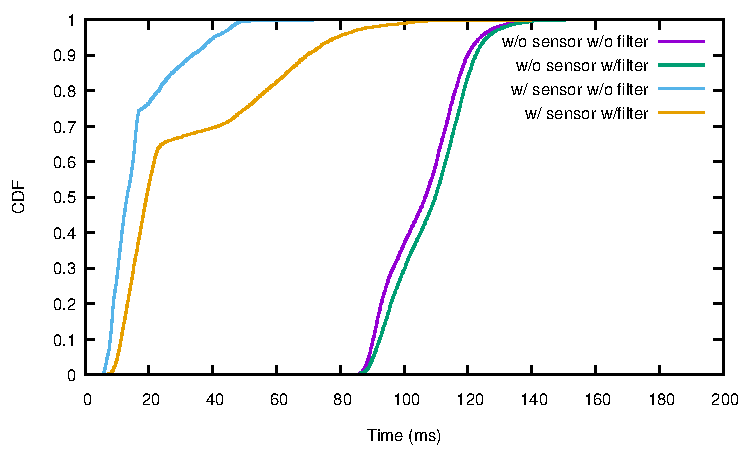
\includegraphics[width=5.2in]{plots/walk_cdf_time.pdf}
\caption{CDF of frame processing time.}
\label{f:cdf_time}
\end{figure}


\ref{f:cdf_time} shows the CDF of the processing time.
It shows that the median of the processing time without sensor and any heuristic filter is 106ms.
Wheather, the median of the processing time with sensor and without heuristic filter is 13ms.
We can improve the processing time 8.15x.
The median of the processing time witt sensor and heuristic filter is 19ms.
Though we can improve the processing time 5.57x with the filter but it increases the accuracy, which we will describe at section \ref{s:acc}

\section{Accuracy}
\label{s:acc}


